\documentclass[../sparc.tex]{subfiles}
\graphicspath{{\subfix{../images/}}}
\begin{document}

%%%%%%%%%%%%%%%%%%%%%%%%%%%%%%%%%%%%%%%%%%%%%%%%%%%%%%%%%%%%%%%%%%%%%%%%%%%%%%%%
\section{Аналогово-цифровое преобразование}

Вы могли заметить в главе \ref{section:analog-ports}, что при считывании с
аналогово порта мы получаем значения от 0 до 1023.  Число 1023 подозрительно
похоже на число 1024, которое в программировании встречается достаточно часто --
не удивительно, ведь 1024 это степень двойки ($2^{10}$).

Если мы проследим дальше этот след, то увидим, что аналоговый порт каким-то
образом перобразует входящий аналоговый сигнал в цифровое (двоичное)
представление, которое мы и видим в программе.

Если мы возьмём 10 бит для хранения информации, то в них мы можем закодировать
$2^{10} = 1024$ разных комбинации из 10 нулей и единиц -- отсюда и максимальное
значение 1023, ведь мы должны учитывать ещё ноль, который также является одним
из возможных значений.

Операцию преобразования аналогового сигнала в цифровой выполняет
\emph{Аналого-Цифровой Преобразователь} (сокращённо ``АЦП'').  В роли АЦП может
выступать отдельная микросхема, или же сам микроконтроллер.  Схематически
аналогово-цифровой преобразователь можно изобразить, как показано на
рис. \ref{fig:adc-schematics}.

По-английски ``АЦП'' -- ``Analog-to-Digital Converter'' (сокращённо ``ADC''.)

\begin{figure}[ht]
  \centering
  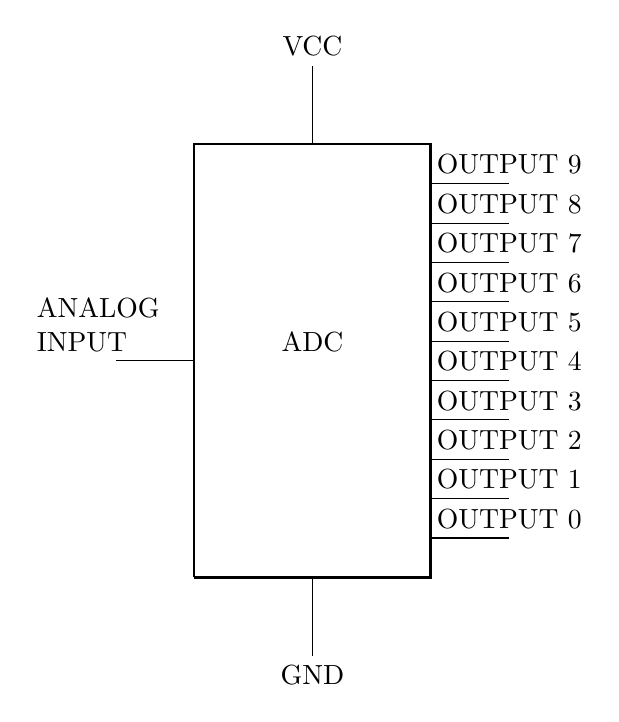
\begin{tikzpicture}
    \draw[thick] (0, 0) -- (0, 5.5) -- (3, 5.5) -- (3, 0) -- (0, 0);
    \draw (1.5, 2.75) node[right, above] {ADC};
    \foreach \n/\y in {0/0.5, 1/1, 2/1.5, 3/2, 4/2.5, 5/3, 6/3.5, 7/4, 8/4.5, 9/5} {
      \draw (3, \y) -- (4, \y) node[right, above] {OUTPUT \n};
    };
    \draw (0, 2.75) -- (-1, 2.75) node[left, above, text width=2cm] {ANALOG INPUT};
    \draw (1.5, 5.5) -- (1.5, 6.5) node[right, above] {VCC};
    \draw (1.5, 0) -- (1.5, -1) node[right, below] {GND};
  \end{tikzpicture}
  \caption{Схематическое изображение аналогово-цифрового преобразователя.}
  \label{fig:adc-schematics}
\end{figure}

На вход АЦП (``ANALOG INPUT'') подаётся аналоговый сигнал, а на выходах
(``OUTPUT 0'' .. ``OUTPUT 9'') кодируется значение входного сигнала в каждый
момент времени в виде набора логических уровней ``HIGH'' (``1'') / ``LOW''
(``0''.)  Самому АЦП требуется также питание -- для этого как раз предназначены
выводы ``VCC'' и ``GND''.

\example { На вход АЦП подаётся 2.5В.  На выходах формируется двоичное значение
  ``1000000000'', что соответствует числу $2^9 = 512$, которое может быть
  получено в программе микроконтроллера. }

Преобразование аналогового сигнала в цифровой внутри АЦП проходит в три этапа:
\begin{enumerate}

\item \textbf{Дискретизация.} Выбираются значения из исходного аналогового сигнала через
  равные временные промежутки (\ref{fig:discretization}.)

  \begin{figure}[h]
    \centering
    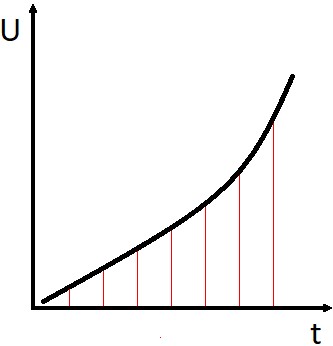
\includegraphics[width=8cm]{discretization}
    \label{fig:discretization}
    \caption{Дискретизация.}
  \end{figure}

  Характеристика, отражающая эти временные промежутки, называется \emph{частотой
  дискретизации}.

\item \textbf{Квантование.} Полученные значения заменяются ближайшим значением из
  набора фиксированных величин -- \emph{уровней квантования}
  (\ref{fig:quantization}.)

  \begin{figure}[h]
    \caption{Квантование.}
    \label{fig:quantization}
    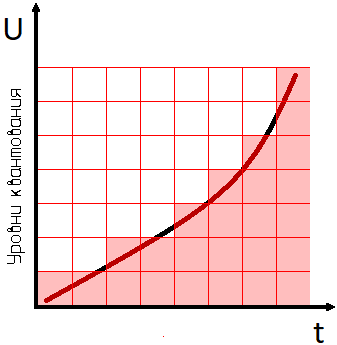
\includegraphics[width=8cm]{quantization}
    \centering
  \end{figure}

\item \textbf{Кодирование.} Квантованным значениям присваивается цифровой код
  (\ref{fig:coding}.)

  \begin{figure}[h]
    \caption{Кодирование.}
    \label{fig:coding}
    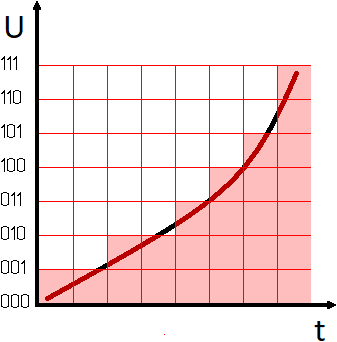
\includegraphics[width=8cm]{coding}
    \centering
  \end{figure}

  Чем выше частота дискретизации и чем больше уровней квантования, тем точнее
  преобразование.

\end{enumerate}

Одной из характеристик АЦП является \emph{разрядность}. Она определяет
количество значений, которое может выдать АЦП. Посмотрим на последний график:
для кодирования значений используется три бита, значит АЦП, описываемый таким
графиком, имеет, соответственно, разрядность 3 бита. То есть $ 2^3 = 8 $, что
равно количеству уровней квантования.

Вот и ответ на поставленный вопрос. АЦП Arduino 10-ти разрядный, $2^{10} = 1024$.
Именно столько значений АЦП Arduino может выдать.

Ещё есть такое устройство как ЦАП - \emph{Цифро-Аналоговый Преобразователь},
который, как нетрудно догадаться, выполняет функцию, обратную функции АЦП -
преобразует цифровой сигнал в аналоговый. Область применения ЦАП и АЦП
достаточно широка: в звуковых и видео- картах, в мониторах, в различной
акустической аппаратуре, в измерительных приборах, и многих других видах
техники.

Стоит упомянуть про 8-битную музыку в древних игровых консолях. Её название
отражает разрядность ЦАП звуковых чипов тех консолей -- 8 бит. Именно такой ЦАП
позволял выдавать тот самый резковатый, хлопающий и шипящий звук.

\end{document}
